%%%%%%%%%%%%%%%%%%%%%%%%%%%%%%%%%%%%%%%%%
% Thin Sectioned Essay
% LaTeX Template
% Version 1.0 (3/8/13)
%
% This template has been downloaded from:
% http://www.LaTeXTemplates.com
%
% Original Author:
% Nicolas Diaz (nsdiaz@uc.cl) with extensive modifications by:
% Vel (vel@latextemplates.com)
%
% License:
% CC BY-NC-SA 3.0 (http://creativecommons.org/licenses/by-nc-sa/3.0/)
%
%%%%%%%%%%%%%%%%%%%%%%%%%%%%%%%%%%%%%%%%%

%----------------------------------------------------------------------------------------
%	PACKAGES AND OTHER DOCUMENT CONFIGURATIONS
%----------------------------------------------------------------------------------------

\documentclass[a4paper, 11pt]{article} % Font size (can be 10pt, 11pt or 12pt) and paper size (remove a4paper for US letter paper)

\usepackage[protrusion=true,expansion=true]{microtype} % Better typography
\usepackage[frenchb]{babel}
\usepackage{graphicx} % Required for including pictures
\usepackage{wrapfig} % Allows in-line images

\usepackage{mathpazo} % Use the Palatino font
\usepackage[utf8]{inputenc} % UTF-8 encoding for input, to get french special characters recognized
\usepackage[T1]{fontenc} % Required for accented characters
\linespread{1.05} % Change line spacing here, Palatino benefits from a slight increase by default

\makeatletter
\renewcommand\@biblabel[1]{\textbf{#1.}} % Change the square brackets for each bibliography item from '[1]' to '1.'
\renewcommand{\@listI}{\itemsep=0pt} % Reduce the space between items in the itemize and enumerate environments and the bibliography

\renewcommand{\maketitle}{ % Customize the title - do not edit title and author name here, see the TITLE block below
\begin{flushright} % Right align
{\LARGE\@title} % Increase the font size of the title

\vspace{50pt} % Some vertical space between the title and author name

{\large\@author} % Author name
\\\@date % Date

\vspace{40pt} % Some vertical space between the author block and abstract
\end{flushright}
}

%----------------------------------------------------------------------------------------
%	TITLE
%----------------------------------------------------------------------------------------

\title{\textbf{Techniques d'optimisation des temps de chargements dans les jeux à monde ouvert}\\ % Title
Ou comment réduire les temps de chargement} % Subtitle

\author{\textsc{Christian NGO \& Jonathan MULLER} % Author
\\{\textit{ESGI - 5ème année IJV}}} % Institution

\date{\today} % Date

%----------------------------------------------------------------------------------------

\begin{document}

\maketitle % Print the title section

%----------------------------------------------------------------------------------------
%	ABSTRACT AND KEYWORDS
%----------------------------------------------------------------------------------------

%\renewcommand{\abstractname}{Summary} % Uncomment to change the name of the abstract to something else

\begin{abstract}
Dans ce mémoire nous verrons comment réduire les temps de chargement des jeux vidéos en se basant à la fois sur les composants de la plateforme cible, sur les techniques de compression, sur l'algorithme et sur le level design.
\end{abstract}

\hspace*{3,6mm}\textit{Mots clefs:} chargement , optimisation , ressources , streaming , jeu % Keywords

\vspace{30pt} % Some vertical space between the abstract and first section

%----------------------------------------------------------------------------------------
%	ESSAY BODY
%----------------------------------------------------------------------------------------

\section*{Introduction}

Les jeux vidéos comportent année après année un nombre grandissant de ressources necessaire pour leur fonctionnement. Des textures aux modèles 3D, le poids de ces ressources augmente tout comme leur nombre, l'augmentation de la taillé mémoire des machines permettant aux créateurs de jeux de charger plus de ressources à la fois. Cependant, augmenter la taille et le nombre des ressources à un prix, celui du temps de chargement. Dans ce mémoire nous verrons comment réduire ces temps de chargement en s'adaptant aux médias qui permettent de stocker les ressources du jeu, en tirant partie des capacités des processeurs, de l'espace disponible et de la mémoire RAM, des différents formats de compression, mais aussi des adaptations de gameplay qui peuvent permettre un chargement transparant pour l'utilisateur.

%------------------------------------------------
\section*{Pourquoi avons nous besoin d'améliorer les temps de chargement ?}
La quantité de mémoire disponible augmente régulièrement sur les postes des utilisateurs, ce qui permet aux concepteurs de jeux de proposer des jeux de plus en plus riches et chargés en éléments graphiques, ce qui demande beaucoup de ressources à créer, stocker, et donc charger. En améliorant des temps de chargement des programmes, nous pouvons faire passer cette quantité de données en mémoire plus rapidement, et donc avoir des jeux qui permettent de jouer rapidement, sans passer de longs instants devant un écran de chargement à plusieurs reprises.

\section*{Comment influencer les temps de chargement}
Les temps de chargement peuvent être influencés de différentes manières.

Nous pouvons améliorer les temps de chargement en utilisant des techniques de stockage qui varient en fonction du média sur lequel le jeu est enregistré. Par exemple, les temps d'accès étant plutôt long sur un cd-rom, il faut veiller à limiter le nombre d'accès aux ressources et penser à charger des elements qui ne seront pas forcèment affichés tout de suite, lors des premiers chargements si la mémoire le permet.

\begin{wrapfigure}{l}{0.4\textwidth}
\begin{center}
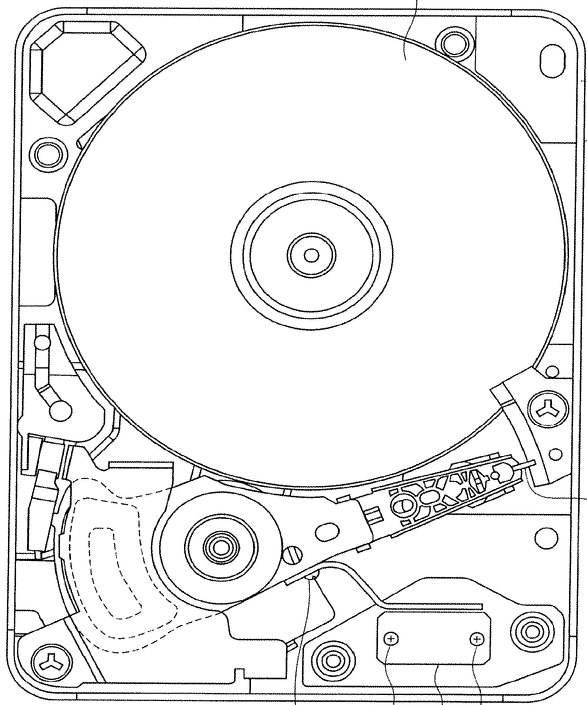
\includegraphics[width=0.38\textwidth]{images/hdd.png}
\end{center}
\caption{Disque dur classique}
\end{wrapfigure}
Au contraire sur un disque SSD, les temps d'accès étant très bas et la capacité de transfert élevée, on pourra séparer les ressources dans des fichiers différents afin de les charger quasiement à la volée.

Les temps de chargement peuvent égallement être réduits en utilisant le processeur pour décompresser des ressources: ainsi le temps necessaire au transfert de la donnée depuis le disque à la mémoire est réduit puisque la donnée est compressée sur le dit disque. Il faut cependant que le mode de compression soit adapté à la puissance du processeur et à la vitesse de transmission du support de stockage.

En modifiant l'algorithme du jeu, nous pouvons aussi influer sur le chargement des données, en évitant par exemple de stocker plusieurs fois des ressources très similaires. Si nous prennons l'exemple des sprites 2D, nous pouvons stocker l'image de base une fois, puis effectuer toutes les déclinaisons de couleurs de manière algorithmique en modifiant la palette de couleurs. De cette façon, nous n'avons qu'à stocker une texture, puis uniquement des palettes de couleurs.

Enfin, une méthode pour cacher les chargements aux joueurs consiste à construire sont level design pour permettre certaines zones "tampons" comme un pont ou un couloir dont le passage est obligatoire pour passer d'une zone à l'autre, et qui va permettre de charger/décharger les zones concernées en tout transparence pour l'utilisateur. Cependant, cette technique est déconseillée puisqu'elle limite la liberté des level-designers en leur imposant des contraintes "techniques".

%------------------------------------------------
%\section*{Optimisation hardware}

%------------------------------------------------
%\section*{Optimisation par compression}

%------------------------------------------------
%\section*{Optimisation par algorithme}

%------------------------------------------------
%\section*{Optimisation par le level design}

%------------------------------------------------

\section*{Conclusion}
Conclusion place-holder

%----------------------------------------------------------------------------------------
%	BIBLIOGRAPHY
%----------------------------------------------------------------------------------------

\bibliographystyle{unsrt}
\bibliography{References}

%----------------------------------------------------------------------------------------

\end{document}
